\documentclass[
  amsfonts,
  amsmath,
  tbtags,
  amssymb,
  aps,
  nobibnotes,
  %% prl,
  twocolumn,
]{revtex4-2}

% imports
\usepackage{appendix}[titletoc]
\usepackage[english]{babel}
\usepackage[justification=centering]{caption}
\usepackage{float}
\usepackage{graphicx}
\usepackage{hyperref}
\usepackage[utf8]{inputenc}
\usepackage{layouts}
\usepackage{optidef}
\usepackage{physics}
\usepackage{setspace}
\usepackage[labelformat=simple]{subcaption}
\usepackage{xcolor}

% configure imports
\DeclareMathOperator*{\argmin}{arg\,min}
\newcommand{\todo}[1]{\textcolor{red}{TODO: #1}}
\definecolor{darkgreen}{RGB}{46, 184, 46}
\newcommand{\half}{\frac{1}{2}}
\newcommand{\R}{\mathbb{R}}
\captionsetup[subfigure]{labelformat=empty, skip=0pt}
\restylefloat{table}
\renewcommand\thesubfigure{(\alph{subfigure})}



\begin{document}

%% TITLE
\title{Robust Quantum Optimal Control}

\author{Thomas Propson}
\email{tcpropson@uchicago.edu}
\affiliation{
  Department of Physics, University of Chicago, Chicago, Illinois 60637, USA
}

\date{\today}


%% ABSTRACT
\begin{abstract}
  %% - 1 + 2 topic importance
  %% - 1 what I have done
  %% - few sentences about primary results
  The ability to engineer high fidelity operations on quantum processors in the presence of
  decoherence and systematic errors remains the primary challenge to achieving quantum advantage.
  Quantum optimal control (QOC) techniques have been developed to mitigate deleterious effects
  by manipulating the time-dependent parameters controlling the system. These techniques often
  target a single error channel and may be incompatible with experimental constraints. 
  In this work, we develop techniques to simultaneously mitigate
  longitudinal relaxation and pure dephasing in a framework that may impose arbitrary
  experimental constraints.
  Optimizing a gate set for a fluxonium qubit as an example, we achieve a factor of 4 increase in
  longitudinal relaxation times and outperform
  existing dynamic decoupling methods in mitigating pure dephasing, achieving
  high fidelity gates in the presence of parameter spreads up to $5\%$.
\end{abstract}

\maketitle


%% S1
\section{Introduction}
%% P1 - general field, lots of citation. cite reviews, original qoc.
%% P2 - exhaustively find all papers, what people have done to address the issues
%% P3 - what we do is. maybe add a rant about how
%% QOC is classical control theory but we've ignored that field
%% P4 - outline
(The field) The field of quantum optimal control (QOC) is concerned
with improving the efficiency and accuracy with which quantum systems
are manipulated.
Early QOC techniques were proposed for nuclear magnetic resonance experiments
\cite{khaneja2005optimal}, and applications now include superconducting
qubits \cite{heeres2017implementing,
  leng2019robust, leung2017speedup, xu2020nonadiabatic},
neutral atoms and ion traps \cite{van2016optimal}, nitrogen-vacancy centers in
diamonds \cite{rembold2020introduction}, and Bose-Einstien condensates
\cite{sorensen2018quantum}.
In quantum control theory, as in classical control theory,
optimization is performed
to minimize an objective function. Relevant for the field
of quantum computation is the task of achieving high fidelity quantum gates.
In this application, the objective function includes contributions from the
gate error associated with the state transfer of the system as well as contributions
due to the decoherence of the system, such as the evolution time of the gate.
The decision variables of the optimization problem are the time-dependent control
parameters, particular to the quantum system, that govern its evolution.

(Existing work) Many analytic and numerical techniques have been developed to control
quantum systems. Analytic methods rely on solving the time-dependent
Schroedinger equation analytically or deriving equations of motion
from a suitable Lagrangian \cite{zhang2020universal, huang2020engineering, han2020experimental,
  xu2020nonadiabatic, carlini2005quantum}. Analytic methods
have been presented to address decoherence in quantum systems.
Considering the dynamical and geometric phases of state
evolution has led to methods for achieving
robustness to dynamical errors and mitigating pure dephasing
\cite{xu2020nonadiabatic, han2020experimental, merrill2014progress}.
Additionally, suitable choices of bases have been proposed that
allow the experimentalist to infer tradeoffs in longitudinal relaxation
and pure dephasing coherence times \cite{huang2020engineering}.
To date, however, no analytical method has been presented
to construct a gate while satisfying arbitrary experimental
constraints. Furthermore, most analytic methods have only
been demonstrated in the two-level approximation and become
cumbersome to solve for larger Hilbert space sizes.

Numerical quantum control techniques have developed in parallel
with analytic frameworks.
Most numerical techniques proposed for QOC are indirect shooting
methods where an initial guess for the control trajectory is forward-simulated,
e.g. under the time-dependent-Schroedinger-equation,
and first-order gradients are computed for a functional evaluated
on the state of the evolved system \cite{leung2017speedup,  goerz2019krotov, doria2011optimal,
  abdelhafez2019gradient, machnes2015gradient, leng2019robust}.
Most techniques formulate the
problem as unconstrained or use
projective gradient methods to enforce constraints
\cite{machnes2015gradient}.
The latter approach relies on constructing
bases for constraint spaces--which is not always feasible--and
may hinder convergence. Methods for mitigating decoherence using numerical
techniques have employed master equation dynamics (citation needed),
Monte Carlo style trajectories \cite{abdelhafez2019gradient},
and proposals have been made to simulate multiple trajectories
\cite{reinhold2019controlling, rembold2020introduction}.

(This work) In this work, we employ state of the art
trajectory optimization methods
to formulate the quantum
optimal control problem as a constrained optimization problem.
The trajectory optimization framework allows us to handle arbitrary
constraints on the evolution of the quantum state. Additionally,
we introduce methods for constructing gates that mitigate longitudinal
relaxation and are robust to experimental errors, and therefore
pure dephasing, the dominant barriers to experimentally
realizing practical quantum computing.

(Outline) As an example, we study the quantum optimal control problem on
the fluxonium qubit presented in \cite{zhang2020universal}.
We describe experimentally realistic constraints and map them to
the trajectory optimization framework. Next, we
outline a method for making the optimization longitudinal
relaxation aware. We achieve a 4x decrease in longitudinal relaxation times
over the baseline gate set.
We present two methods for achieving robustness to pure dephasing
and compare them to existing dynamic decoupling methods. We find that
the methods we employ outperform dynamic decoupling, producing
high fidelity gates at system parameter spreads of $5\%$.


%% S2
\section{QOC + AL-iLQR}
(QOC Problem Statement) Here we introduce the notation
we will use throughout the paper,
review the quantum optimal control problem statement,
and introduce the trajectory optimization framework.
Quantum optimal control concerns the evolution of
a quantum state $\ket{\psi(t)}$ governed by the time-dependent
Schroedinger equation (TDSE)
\label{eq:tdse}
\begin{align}
  \frac{d}{dt} \ket{\psi(t)} &= -\frac{i}{\hbar} H(u(t), t) \ket{\psi(t)}
\end{align}
The evolution is sometimes cast with the evolution
of a density matrix under the Lindblad master equation to
model the decoherence of the state explicitly. The Hamiltonian
has an arbitrary dependence on the possibly multi-valued controls $u(t)$.
The controls are so called because they are the means the experimentalist has to
act on the system.

Numerical quantum optimal control techniques make
the problem tractable by discretizing the problem into $N$
knot points (time steps). Typical integration techniques for the TDSE include
approximating unitary propagators as well as explicit integration methods,
such as Runge-Kutta, of the form
$\ket{\psi_{k + 1}} \approx \ket{\psi_{k}} + \frac{d}{dt} \ket{\psi_{k}} \cdot \Delta t_{k}$

Quantum optimal control seeks the control
parameters that minimize a functional $J(u(t))$.
In the simplest case the functional is
$J = 1 - {\lvert \braket{\psi_{f} \lvert \psi_{N}(u(t))} \rvert}^{2}$
the infidelity between the inital state evolved
to the final knot point ($\ket{\psi_{N}(u(t))}$)
and the target state ($\ket{\psi_{f}}$). In general
$J$ is a linear combinaion of cost functions on the state, e.g.
forbidden-state occupation, as well as
cost functions on the controls, e.g. the norm of the control amplitudes
\cite{leung2017speedup}. Typical quantum optimal control
algorithms employ automatic differentiation
to compute first order information for the functional ($\nabla_{u} J(u)$).
They employ a first-order optimizer to minimize $J$ with respect to $u$.

(AL-iLQR Problem Statement) The trajectory optimization
literature solves a more general class of non-linear programs that resemble
the quantum optimal control problem. The quantum optimal control
problem is a specific case of the linear quadratic regulator (LQR).
LQR is so called because the dynamics are linear in the state and
the functional is quadratic in the state. In the LQR formulation
the same functional is evaluated at each knot point
\begin{equation}
  J_{\textrm{iLQR}} = \tilde{x}_{N}^{T} Q_{N} \tilde{x}_{N}
  + \sum_{k = 0}^{N - 1} \tilde{x}_{k}^{T} Q_{k} \tilde{x}_{k} + u_{k}^{T} R_{k} u_{k}
\end{equation}
where $\tilde{x}_{k} = x_{k} - x_{f}$ is the difference between the state
at knot point $k$ and final state, $u_{k}$ are the controls,
and $Q_{k}, R_{k}$ are matrices that define the penalty metric.
The state is propagated using a dynamics function
$x_{k + 1} = f(x_{k}, u_{k}, t_{k}, \Delta t_{k})$.
In the case of quantum optimal control $\ket{\psi_{k}} \subseteq x_{k}$
and $f$ encodes the TDSE dynamics. In the following
we refer to $\ket{\psi}$ as the state. We refer to $x$ and $u$ as
the augmented state and augmented controls, respectively.

The advantage of the LQR formulation
is that there exists a dynamic programming algorithm to compute the
optimal update to the augmented controls ($u_{k}$) which minimizes the functional
($J_{\textrm{iLQR}, k}$) for each knot point. This algorithm proceeds by deriving a
recurrence relation between knot points $k$ and $k + 1$ for the optimal
feedback law--known as the Ricatti recursion (see Appendix). The
iterative LQR (iLQR) algorithm computes $J_{\textrm{iLQR}}$
and applies the Ricatti recursion to all knot points on multiple
executions.

In order to incorporate constraints we employ
the augmented Lagrangian method. Constraints are contributions
to the functional of arbitrary form $c_{k}(x_{k}, u_{k})$ which are
zero or negative when the constraint is satisfied. The AL-iLQR
method associates a penalty multiplier with the functional
that estimates the constraint's Lagrange multiplier.
The algorithm updates the penalty multiplier between
iLQR executions. In this scheme the functional takes the form
\begin{equation}
  \begin{aligned}
    J_{\textrm{AL-iLQR}} = \ &(\lambda_{k} + \frac{1}{2}I_{\mu_{k}} c_{k}(x_{k}, u_{k}))^{T} c_{k}(x_{k}, u_{k})\\
    &+ J_{\textrm{iLQR}}
  \end{aligned}
\end{equation}
where $\lambda_{k}$ is a Lagrange multiplier and $I_{\mu_{k}}$ is a penalty matrix
with $\mu_{k}$ along the diagonal.
$\lambda_{k}$ and $\mu_{k}$ are updated after each augmented Lagrangian iteration according to
\begin{align}
  \lambda_{k_{i}} &\gets \max(0, \lambda_{k_{i}} + \mu_{k_{i}} c_{k_{i}}(x_{k}^{*}, u_{k}^{*}))\\
  \mu_{k_{i}} &\gets \phi \mu_{k_{i}}
\end{align}
where $x^{*}, u^{*}$ are the optimal augmented state and augmented controls from the iLQR execution,
$i$ indicates the $i$-th constraint functional,
and $\phi$ is a hyperparameter. With this updated form of the cost
functional there still exists a recurrence relation to calculate the optimal control
updates, see \cite{howell2019altro}.


%% F4.1
\begin{figure}[ht]
  \begin{subfigure}{\linewidth}
    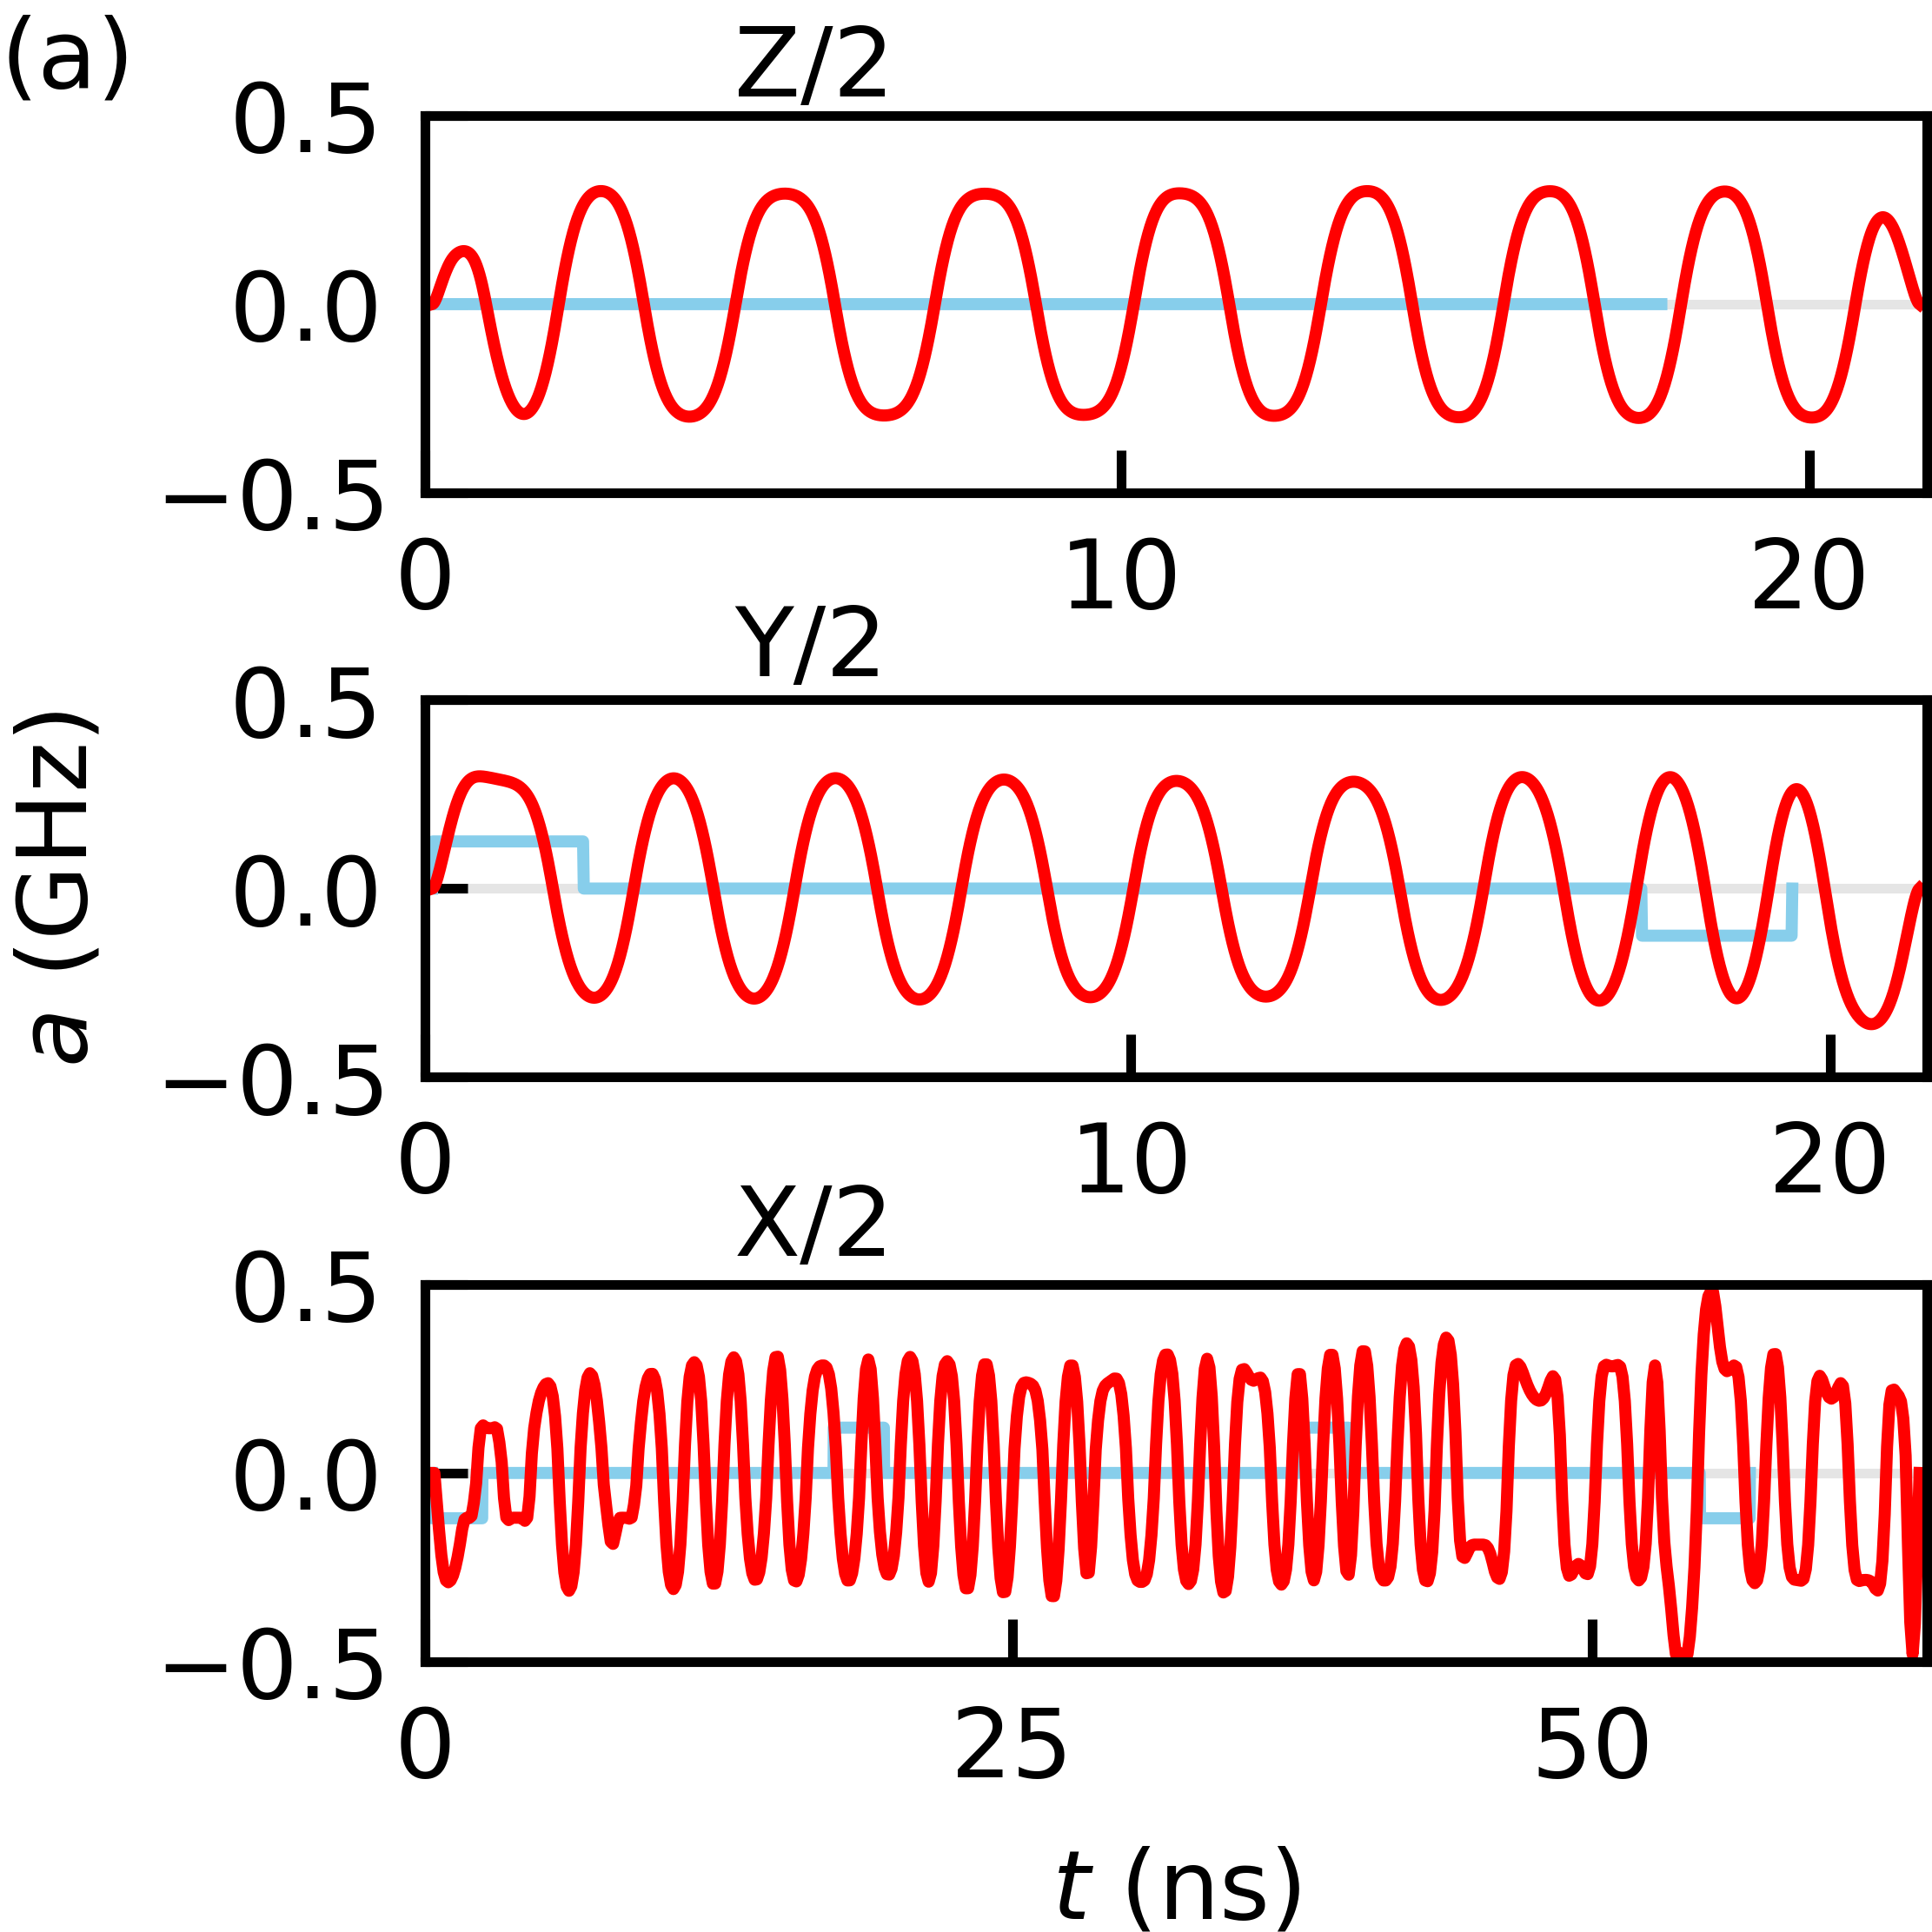
\includegraphics[width=\linewidth]{assets/f1a.png}
  \end{subfigure}
  \begin{subfigure}{\linewidth}
    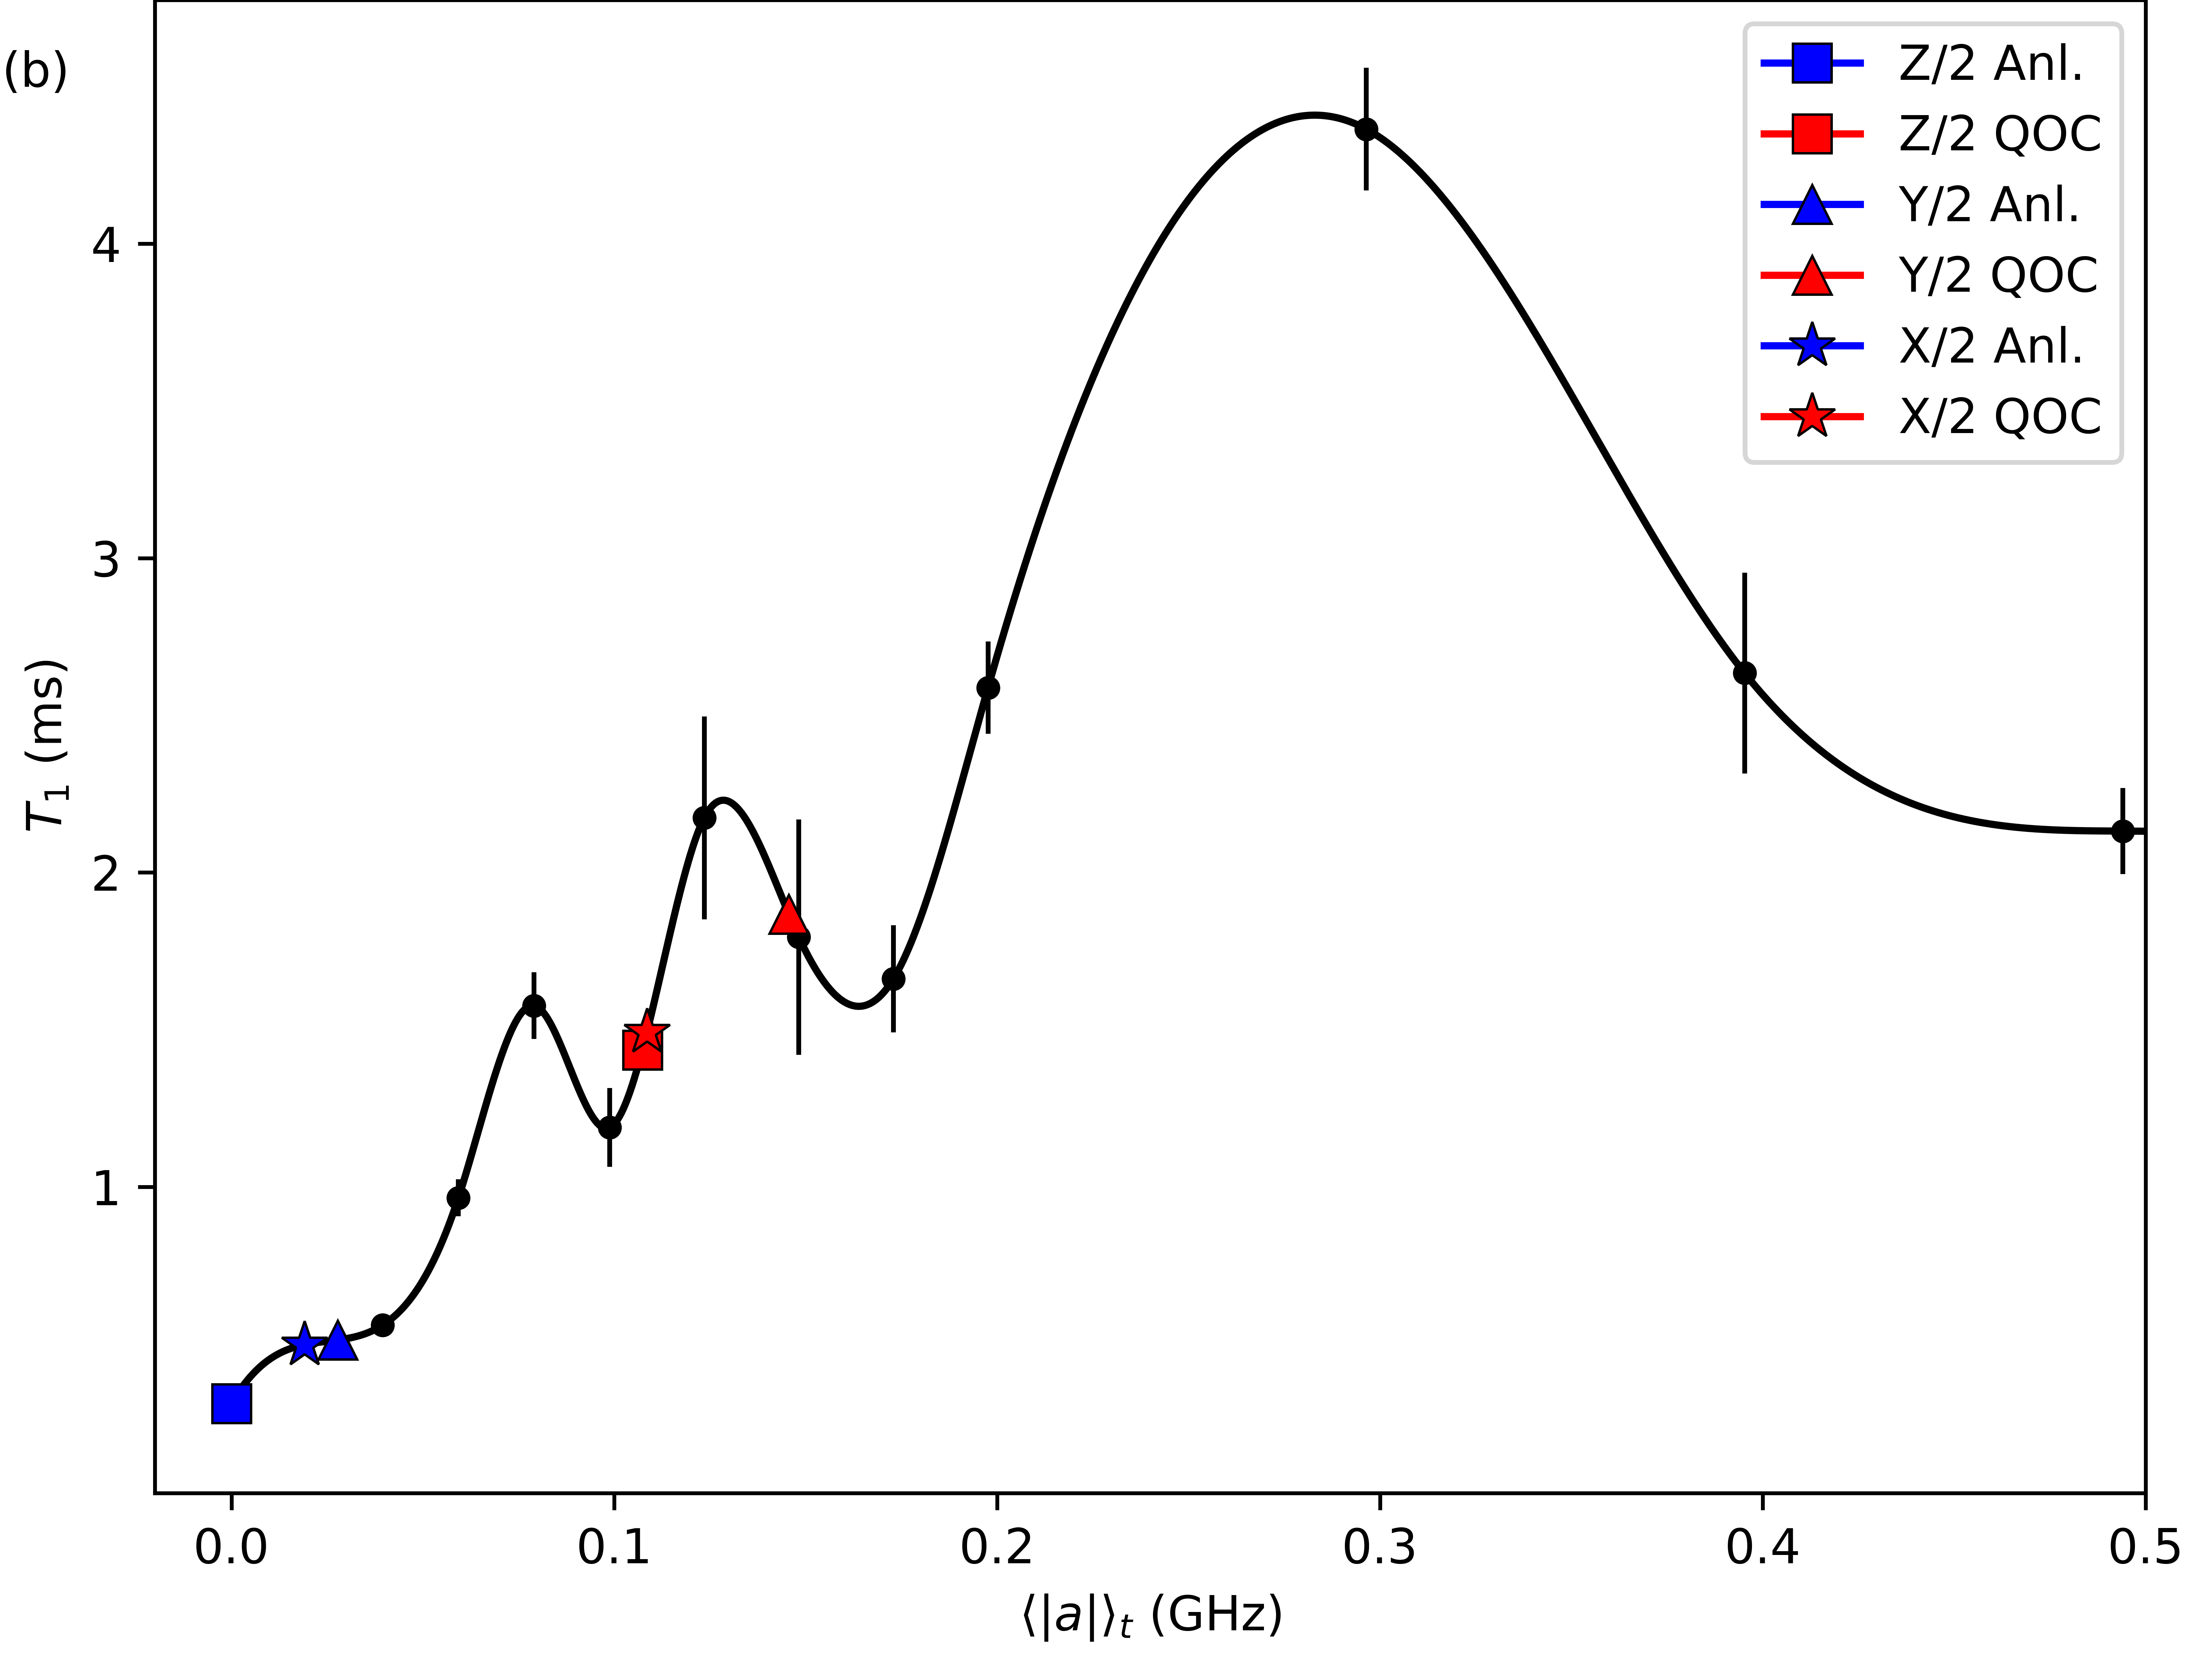
\includegraphics[width=\linewidth]{assets/f1b.png}
  \end{subfigure}
  \begin{subfigure}{\linewidth}
    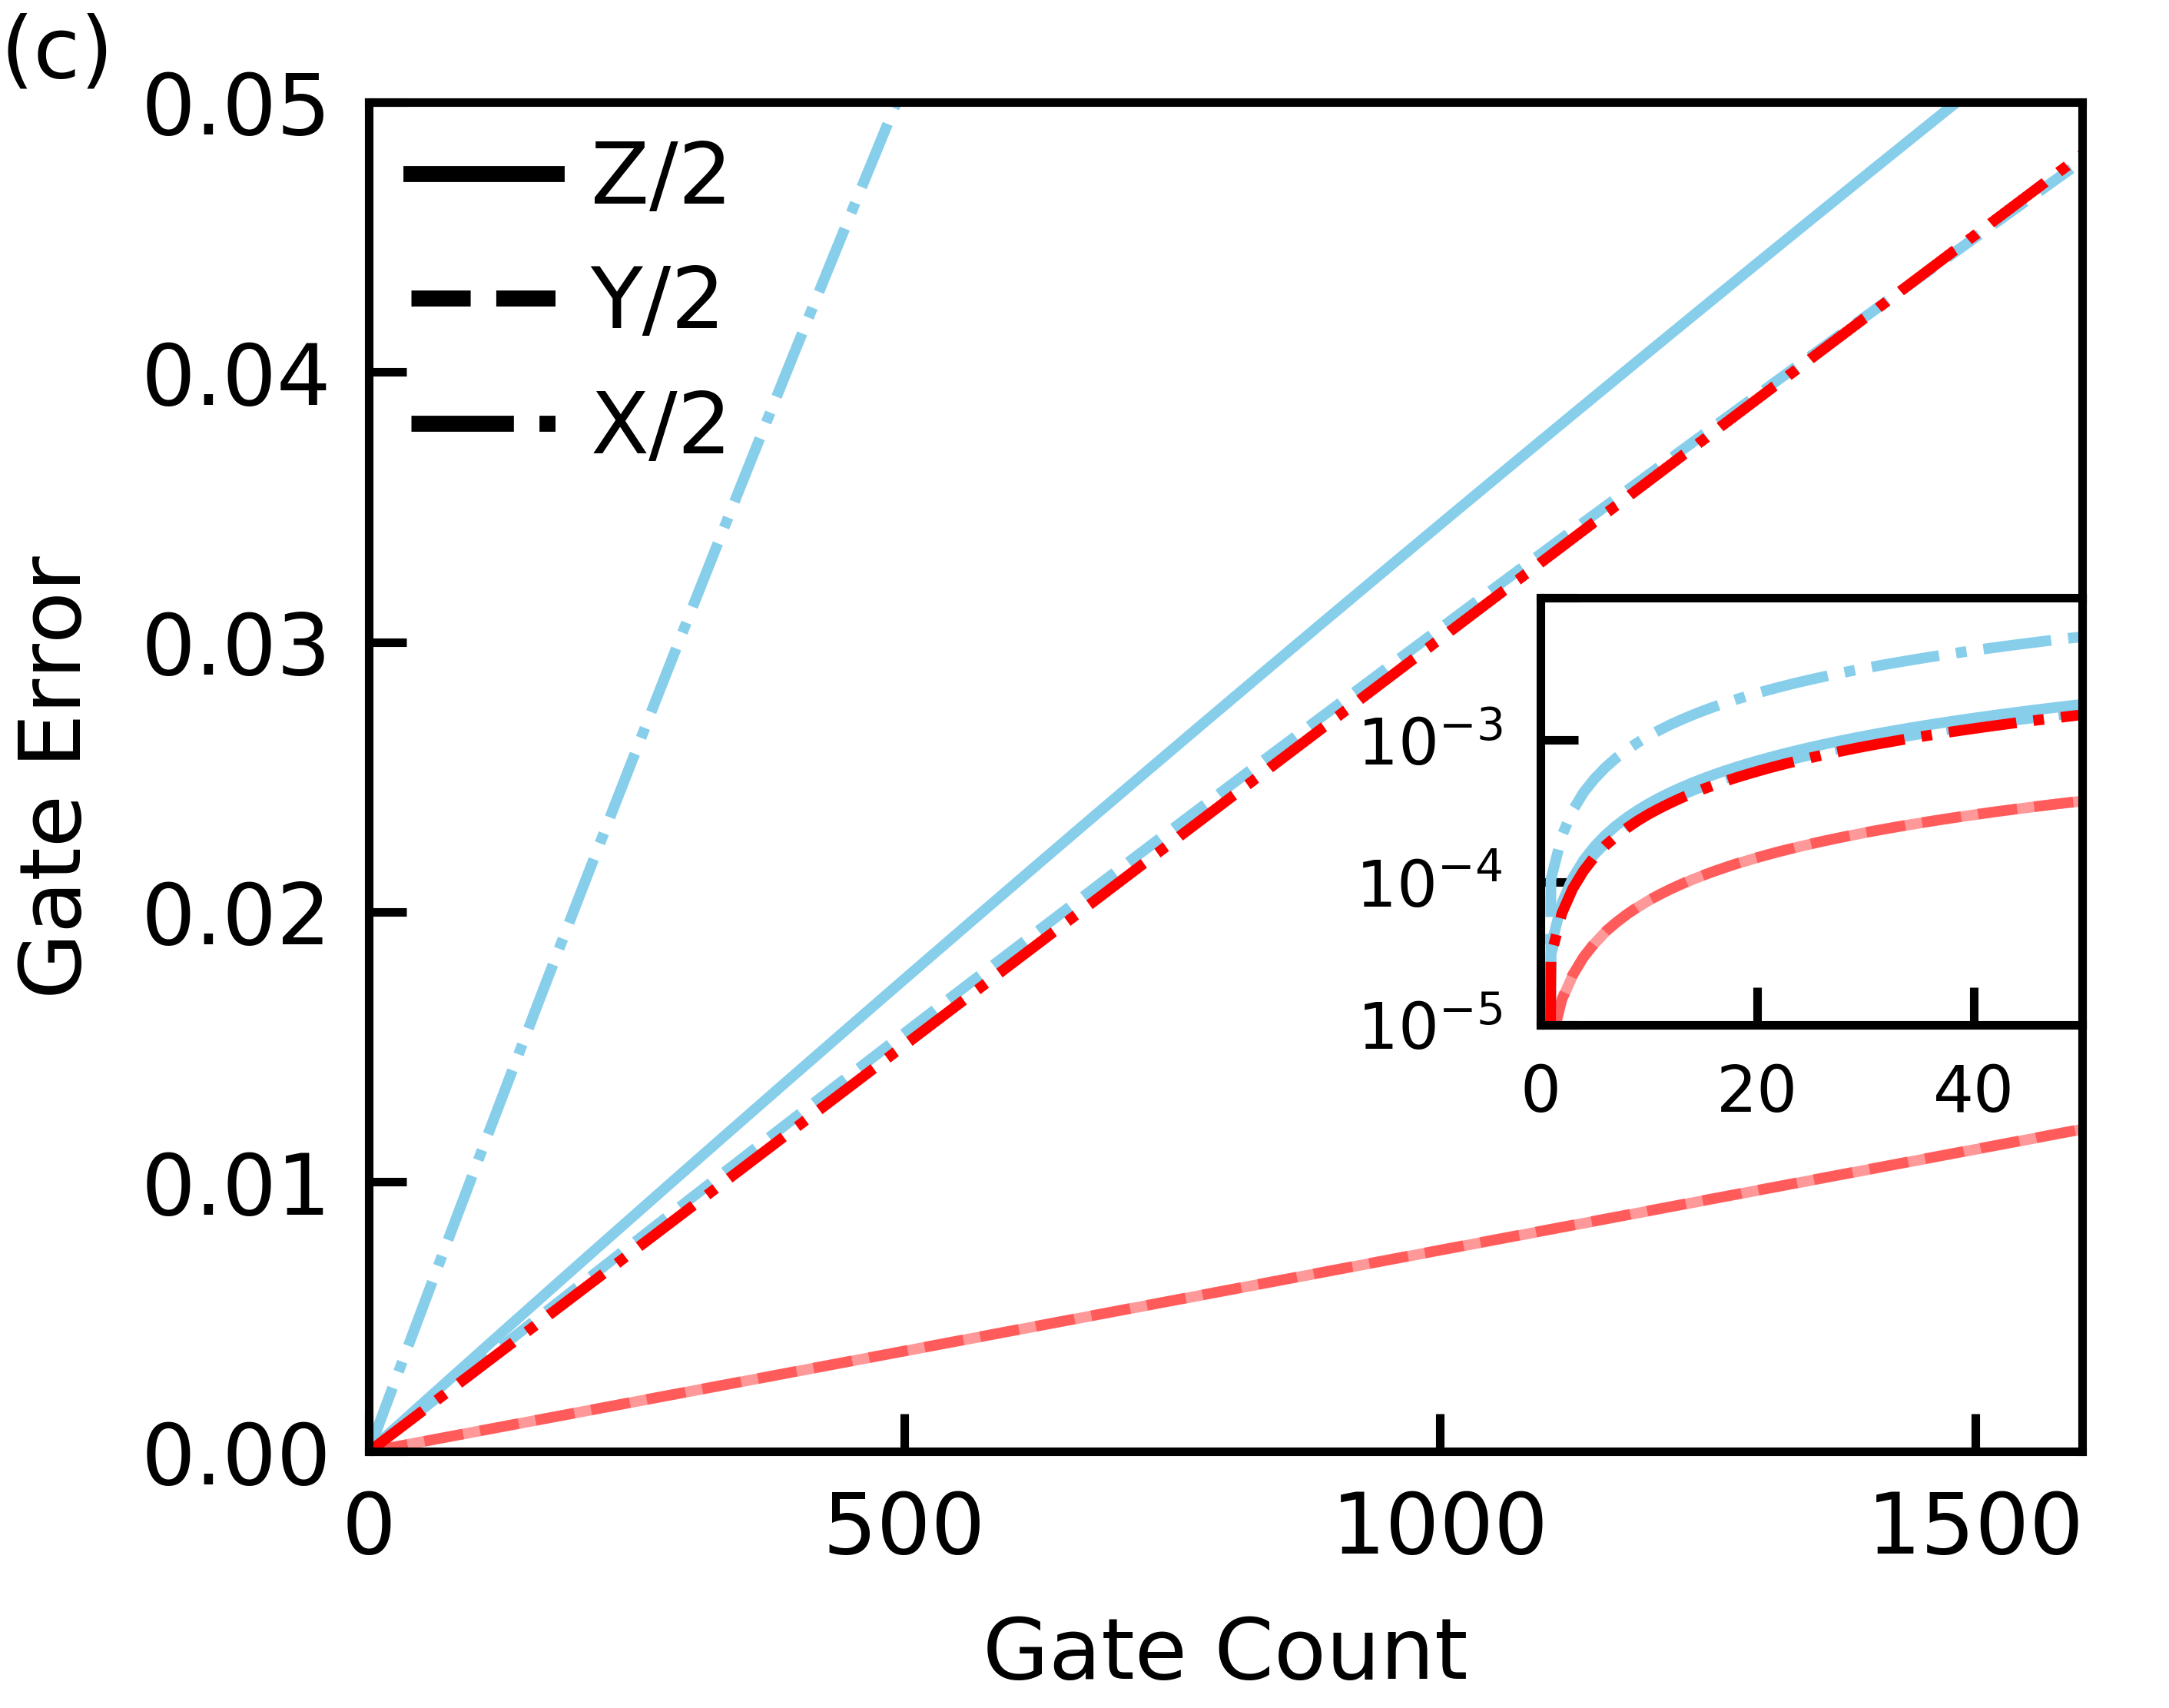
\includegraphics[width=\linewidth]{assets/f1c.png}
  \end{subfigure}
  \caption{(a) $T_{1}$ optimized gates (orange) and analytic gates (blue). (b) Master equation simulation with $T_{1}$ dissipation
    for all gates, over the course of concatenated gate applications. (c) $T_{1}$ interpolation function used in optimization
    and the corresponding $T_{1}$ times for the average absolute amplitude of each gate.}
\end{figure}


%% S3
\section{QOC on the Fluxonium}
(Fluxonium Device) In the following we study
the quantum optimal control problem on the fluxonium qubit.
In the two-level
approximation the system Hamiltonian takes the form
\label{eq:hamiltonian}
\begin{align}
  H/h &= \omega_{q} \frac{\sigma_{z}}{2} + a(t) \frac{\sigma_{x}}{2}
\end{align}
where $\omega_{q}$ is the qubit frequency at the flux frustration point,
$a$ is the flux drive amplitude, $h$ is Planck's constant, and $\sigma_{x}, \sigma_{y}$
are Pauli matrices. The flux amplitude $a$ is experimentally
realized by modulating the flux 
threading the device ($\Phi_{\textrm{ext}}$).
The flux amplitude is obtained from the external flux by
$a = 4 \pi \braket{g \lvert \hat{\phi} \rvert e} \rvert_{0.5 \Phi_{0}} E_{L}
\delta \Phi_{\textrm{ext}} / (h \Phi_{0})$
where $\hat{\phi}$ is the phase operator, $E_{L}$ is the characteristic inductance energy, $\Phi_{0}$
is a flux quantum, and
$\delta \Phi_{\textrm{ext}} = \Phi_{\textrm{ext}} - 0.5 \Phi_{0}$ is the flux
offset from the flux frustration point.

In the following we compare the gates found with our methods
to the $X/2, Y/2, Z/2$ gates reported in \cite{zhang2020universal}
for the same device. Note that $Y/2$ and arbitrary $Z$ rotations
are sufficient for universal computation.
%% TODO: list device parameters

(Constraints) We now outline the constraints that we require each gate
to obey.
We require $a(t = 0) = a(t = t_{N}) = 0$.
This constraint ensures gates may be concatenated arbitrarily without
inducing AWG ringing due to high-frequency transitions.
Furthermore, we require $\int_{0}^{t_{N}} a(t) dt = 0$. This
constraint ensures the pulse has zero net flux, mitigating
the hysteresis ubiquitous in flux bias lines.
%% TODO: See ref. 28 in Helin paper
We require $-300 \textrm{MHz} \le a(t) \le 300 \textrm{MHz}$
to ensure the two-level approximation \ref{eq:hamiltonian}
remains valid. Additionally, we require that each gate achieves
the desired state transition $\braket{\psi_{f} \lvert \psi_{N}} = 1$.
In addition to these constraints we penalize the norm
of the first and second derivatives of the flux amplitude
to mitigate AWG ringing.

The optimization is performed over the second derivative of the flux amplitude
($\frac{d^{2}}{dt^{2}} a(t)$) which is contained in the
augmented control vector. The first derivative
($\frac{d}{dt} a(t)$), proportional ($a(t)$), and integral ($\int a(t)$)
flux amplitude terms
are contained in the augmented state vector. They are obtained from
the second derivative of the flux amplitude by
integration in the dynamics function $f$.
Both the zero net flux and target quantum state constraint
are then handled by ensuring the augmented final state is
reached $x_{N} - x_{f} = 0$.
The equality and inequality constraints on $a(t)$ are handled
with a bound constraint.
%% TODO: probably want to list equations for the constraints

($T_{1}$ and $T_{\phi}$ noise)
In addition to optimizing the cost functional to achieve a gate
that obeys experimental constraints and has a high simulated fidelity,
we also want to make the gate robust to noise that affects the experimental
gate fidelity. Decoherence of the quantum state due to external noise
is typically modeled by two phenomena: longitudinal relaxation and pure dephasing.
They are modeled using their $1/e$ decay times $T_{1}$ and $T_{\phi}$ respectively
(see Appendix).
The main contributions to longitudinal relaxation in our
device are dielectric loss in the capacitor, resistive loss in the inductor,
and Purcell loss. The main contributions to pure dephasing in our
device are $1/f$ flux noise and decay via charge and flux coupling
to the control lines.

Dissipation to the thermal bath via longitudinal
relaxation is an irreversible process
that results in information loss.
Converesely, pure dephasing is a reversible process.
There is a tradeoff between the two decoherence processes. In the case of white
noise we have that the sum of the noise weights $W_{1}$ and $W_{\phi}$
is constant \cite{huang2020engineering}.
Our device achieves its best pure dephasing
protection at the flux frustration point
$T_{2e}(\Phi_{\textrm{ext}} = 0.5 \Phi_{0}) \sim 300 \mu\textrm{s}$
where the qubit frequency is first-order insensitive to changes in flux.
It becomes more succeptable to pure dephasing as the flux is tuned away from the flux
frustration point. Conversely, $T_{1}$ is at a minimum
at the flux frustration point $T_{1}(0.5 \Phi_{0}) = 0.315$ms,
and increases away from the flux frustration point
$T_{1}(0.43 \Phi_{0}) = 4.3$ms. Given the nature
of the decay processes and the tradeoff, we choose
to maximize the longitudinal relaxation time ($T_{1}$)
over the gate duration
and employ robust control techniques to mitigate
pure dephasing.
%% TODO: See fig. 3 in Helin paper


%% S4
\section{Longitudinal Relaxation Awareness}
(Strategy) We seek to minimize the probability
that the qubit decays as a result of longitudinal
relaxation. To this end we add the
longitudinal relaxation probability
to the augmented state vector
\begin{equation}
  P_{1}(t) = \int_{0}^{t} \gamma_{1}(a(t^{\prime})) dt^{\prime}
\end{equation}
where $\gamma_{1} = T_{1}^{-1}$. Setting the target
longitudinal relaxation probability to 0 results in
a quadratic cost at each knot point
of the form ${\lvert P_{1}(t_{k}) \rvert}^{2}$.

$\gamma_{1}(a_{k})$
is obtained at each knot point by evaluating
a spline interpolant fit to
experimentally obtained data of the form
$\{(\Phi_{\textrm{ext}}, T_{1})\}$.
$\Phi_{\textrm{ext}}$ is a function of $a_{k}$
with the inverse of the relation given in section 3.
Calculating $T_{1}$ directly from theoretical
considerations requires many high-dimensional
eigendecompositions, which
is computationally expensive. Additionally,
$T_{1}$ values are known to fluctuate greatly
with laboratory temperatures \cite{klimov2018fluctuations}.
Interpolating $T_{1}$ from experimental data increases
the fridge truth of the simulation.

Furthermore, the probability of longitudinal 
relaxation is dependent on the gate duration $t_{N}$.
We allow the optimizer to tune the gate duration by
adding the time step between knot points $\Delta t_{k}$
to the augmented control vector $u_{k}$.
Promoting $\Delta t_{k}$ to a decision variable, rather
than the number of knot points $N$, preserves the
Markovian decision structure of the trajectory
optimization problem. To ensure numerical
integration accuracy is maintained we add a bound
constraint at each knot point
$5\textrm{e-}3 \ \textrm{ns} \le
\Delta t_{k} \le 2\textrm{e-}2 \ \textrm{ns}$.
Note that this bound constraint is allowed to be
broken for intermediate iterations of the optimization,
so we use the absolute value of the time step
$\lvert \Delta t_{k} \rvert$ to ensure that it is non-negative.

(Results) We achieve a factor of 2.5 decrease in the probability
of longitudinal relaxation from the analytic gates we benchmark
against. We simulate the performance of the gates using the
Lindblad master equation (see Appendix). We repeatedly apply the basis gates
and measure the fidelity of the resulting state as a function
of time as shown in Fig. 1.

%% T4.1
%% TODO: Maybe best for appendix.
%% TOOD: Maybe add some commentary about why we see more speedup
%% for Z/2 and X/2 than Y/2. In particular I think this is because of the
%% long idle times at the flux frustration point for Z/2 and X/2. It
%% might be a more fair comparison to show gates that have better T1s
%% and as good flux noise mitigation.

\begin{table}[ht]
  \begin{tabular}{c | c | c | c}
    & Analytic  & QOC &\\
    Gate & $P_{1}\ (10^{-5})$ & $P_{1}\ (10^{-5})$ & Speedup\\
    \hline
    Z/2 & 5.745 & 1.469 & 3.911\\
    Y/2 & 5.253 & 1.400 & 3.752\\
    X/2 & 16.251 & 6.946 & 2.340\\
  \end{tabular}
  \caption{Probability of longitudinal relaxation for each gate
    evaluated at the gate's duration.}
\end{table}


%% F5.1
\begin{figure}[ht]
  \begin{subfigure}{\linewidth}
    \label{fig:5.1:a}
    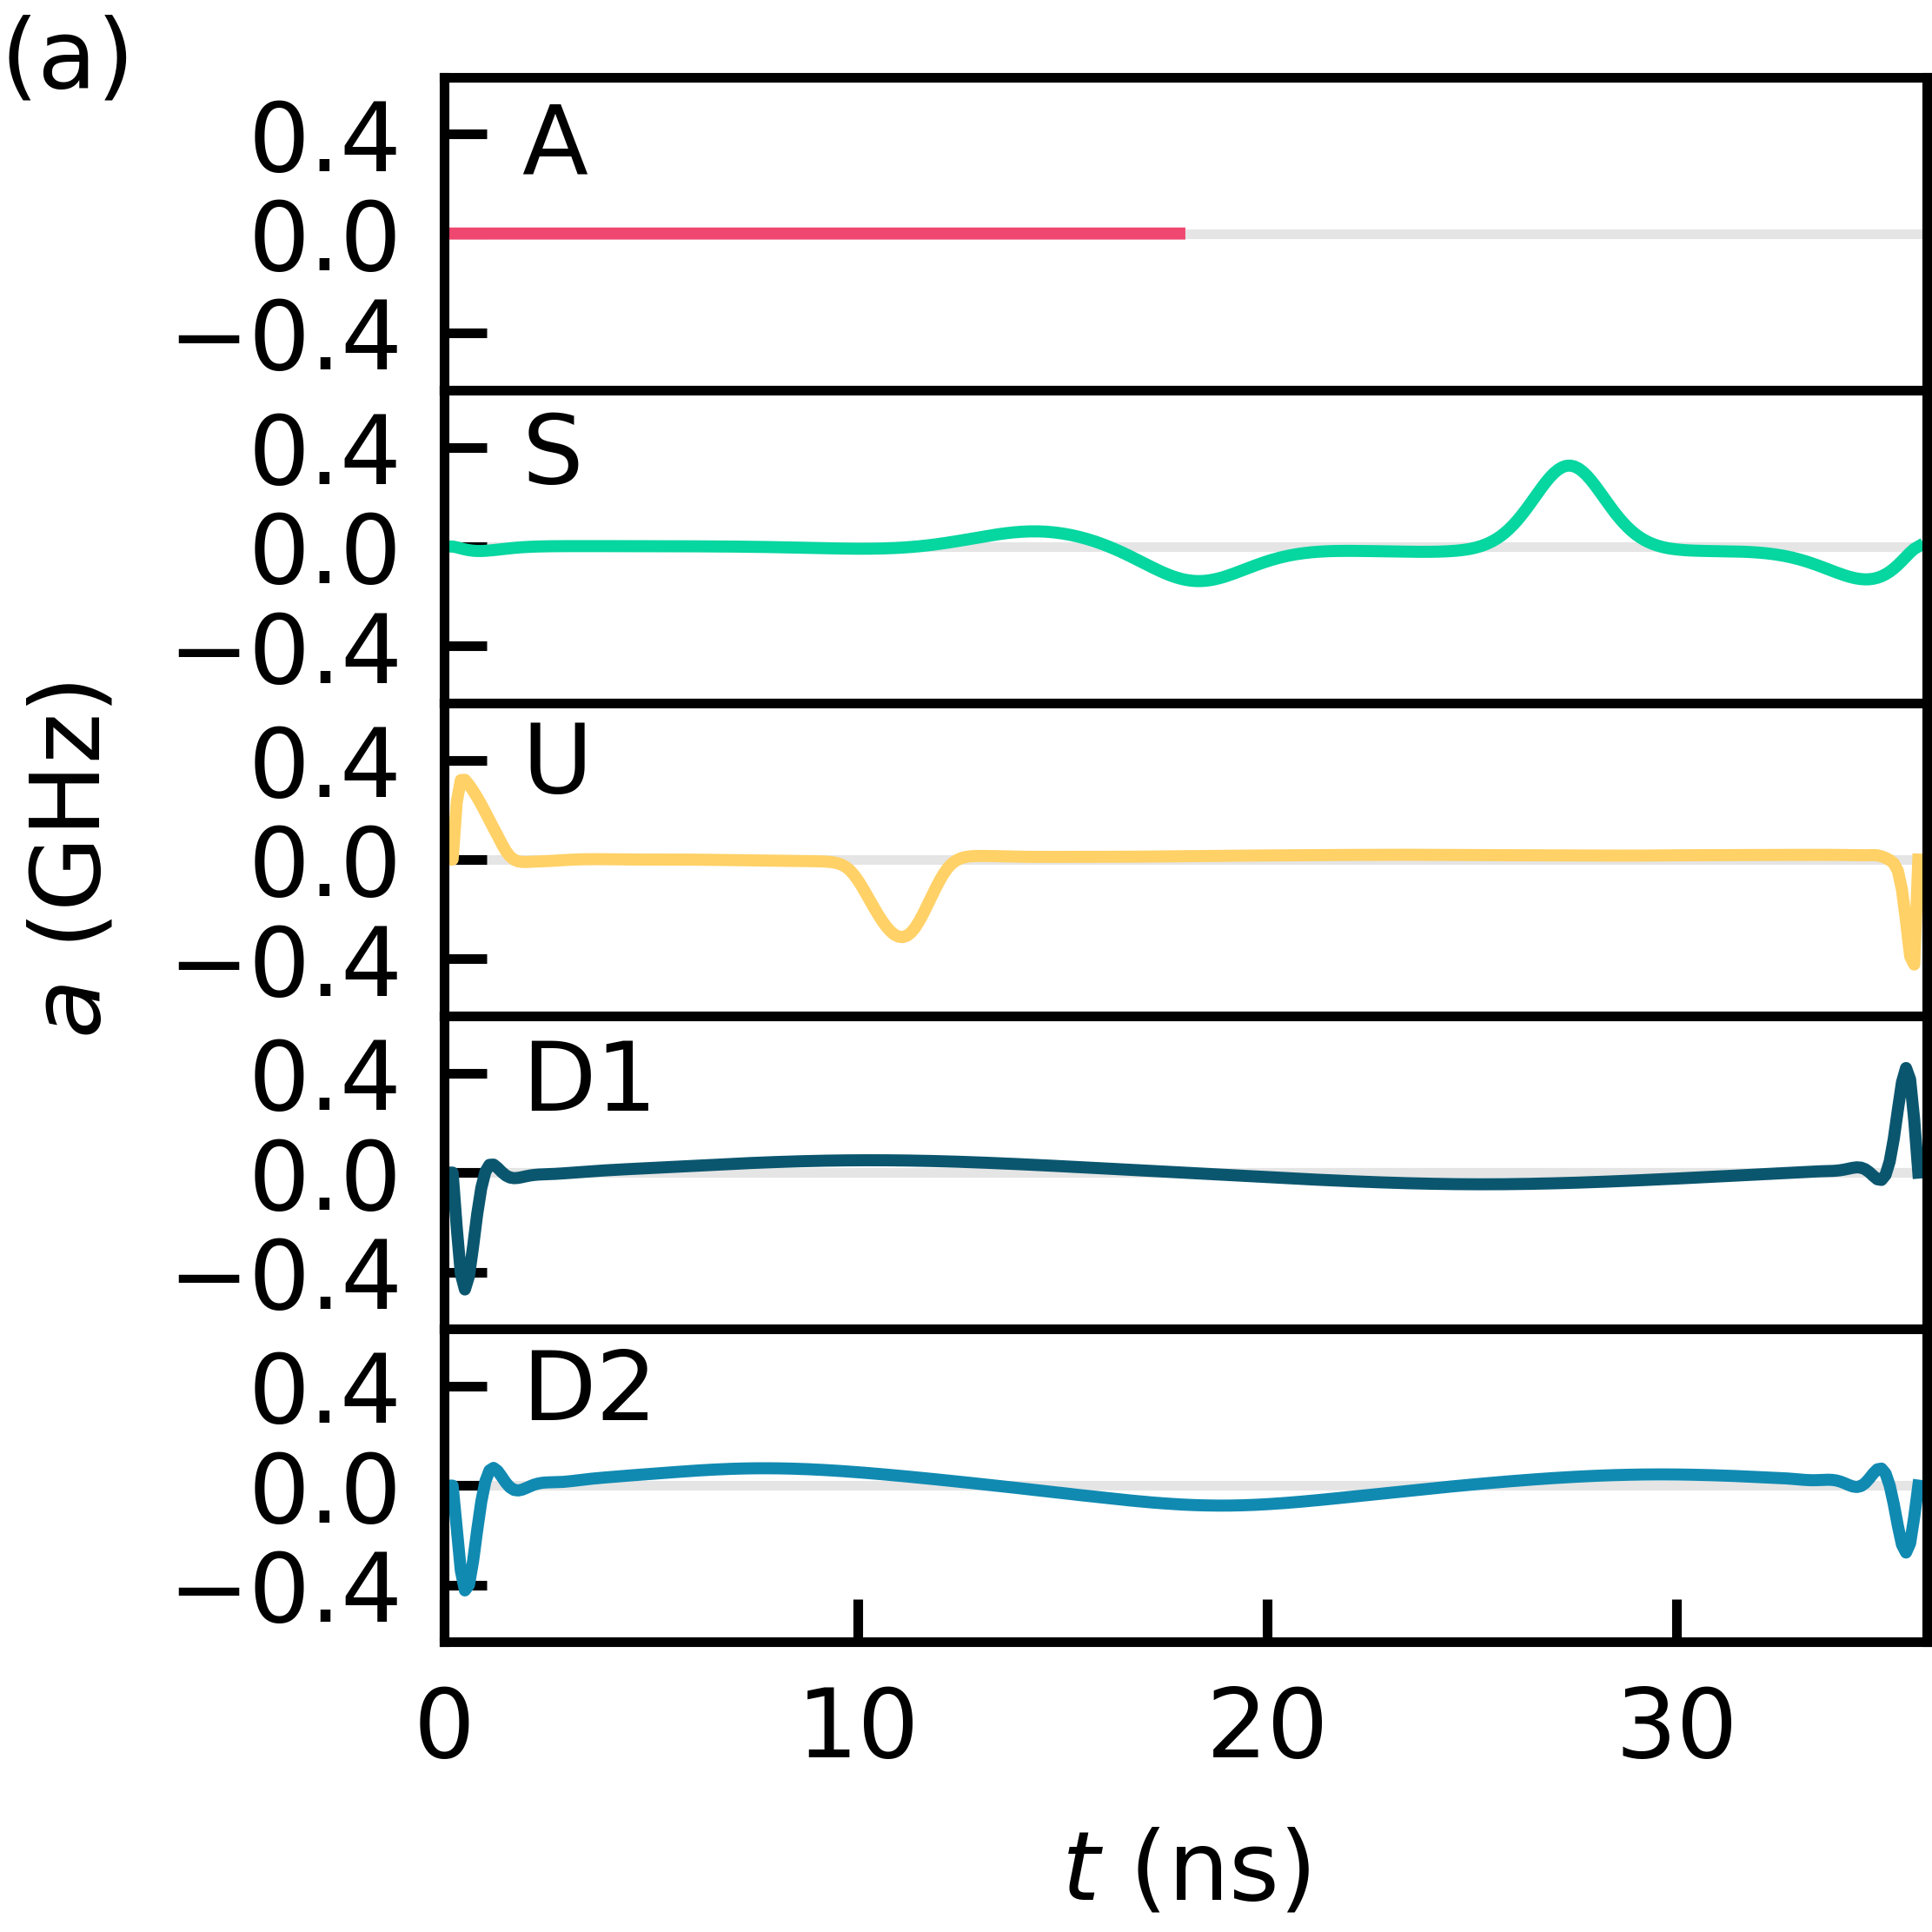
\includegraphics[width=\linewidth]{assets/f2a.png}
  \end{subfigure}
  
  \begin{subfigure}{\linewidth}
    \label{fig:5.1:b}
    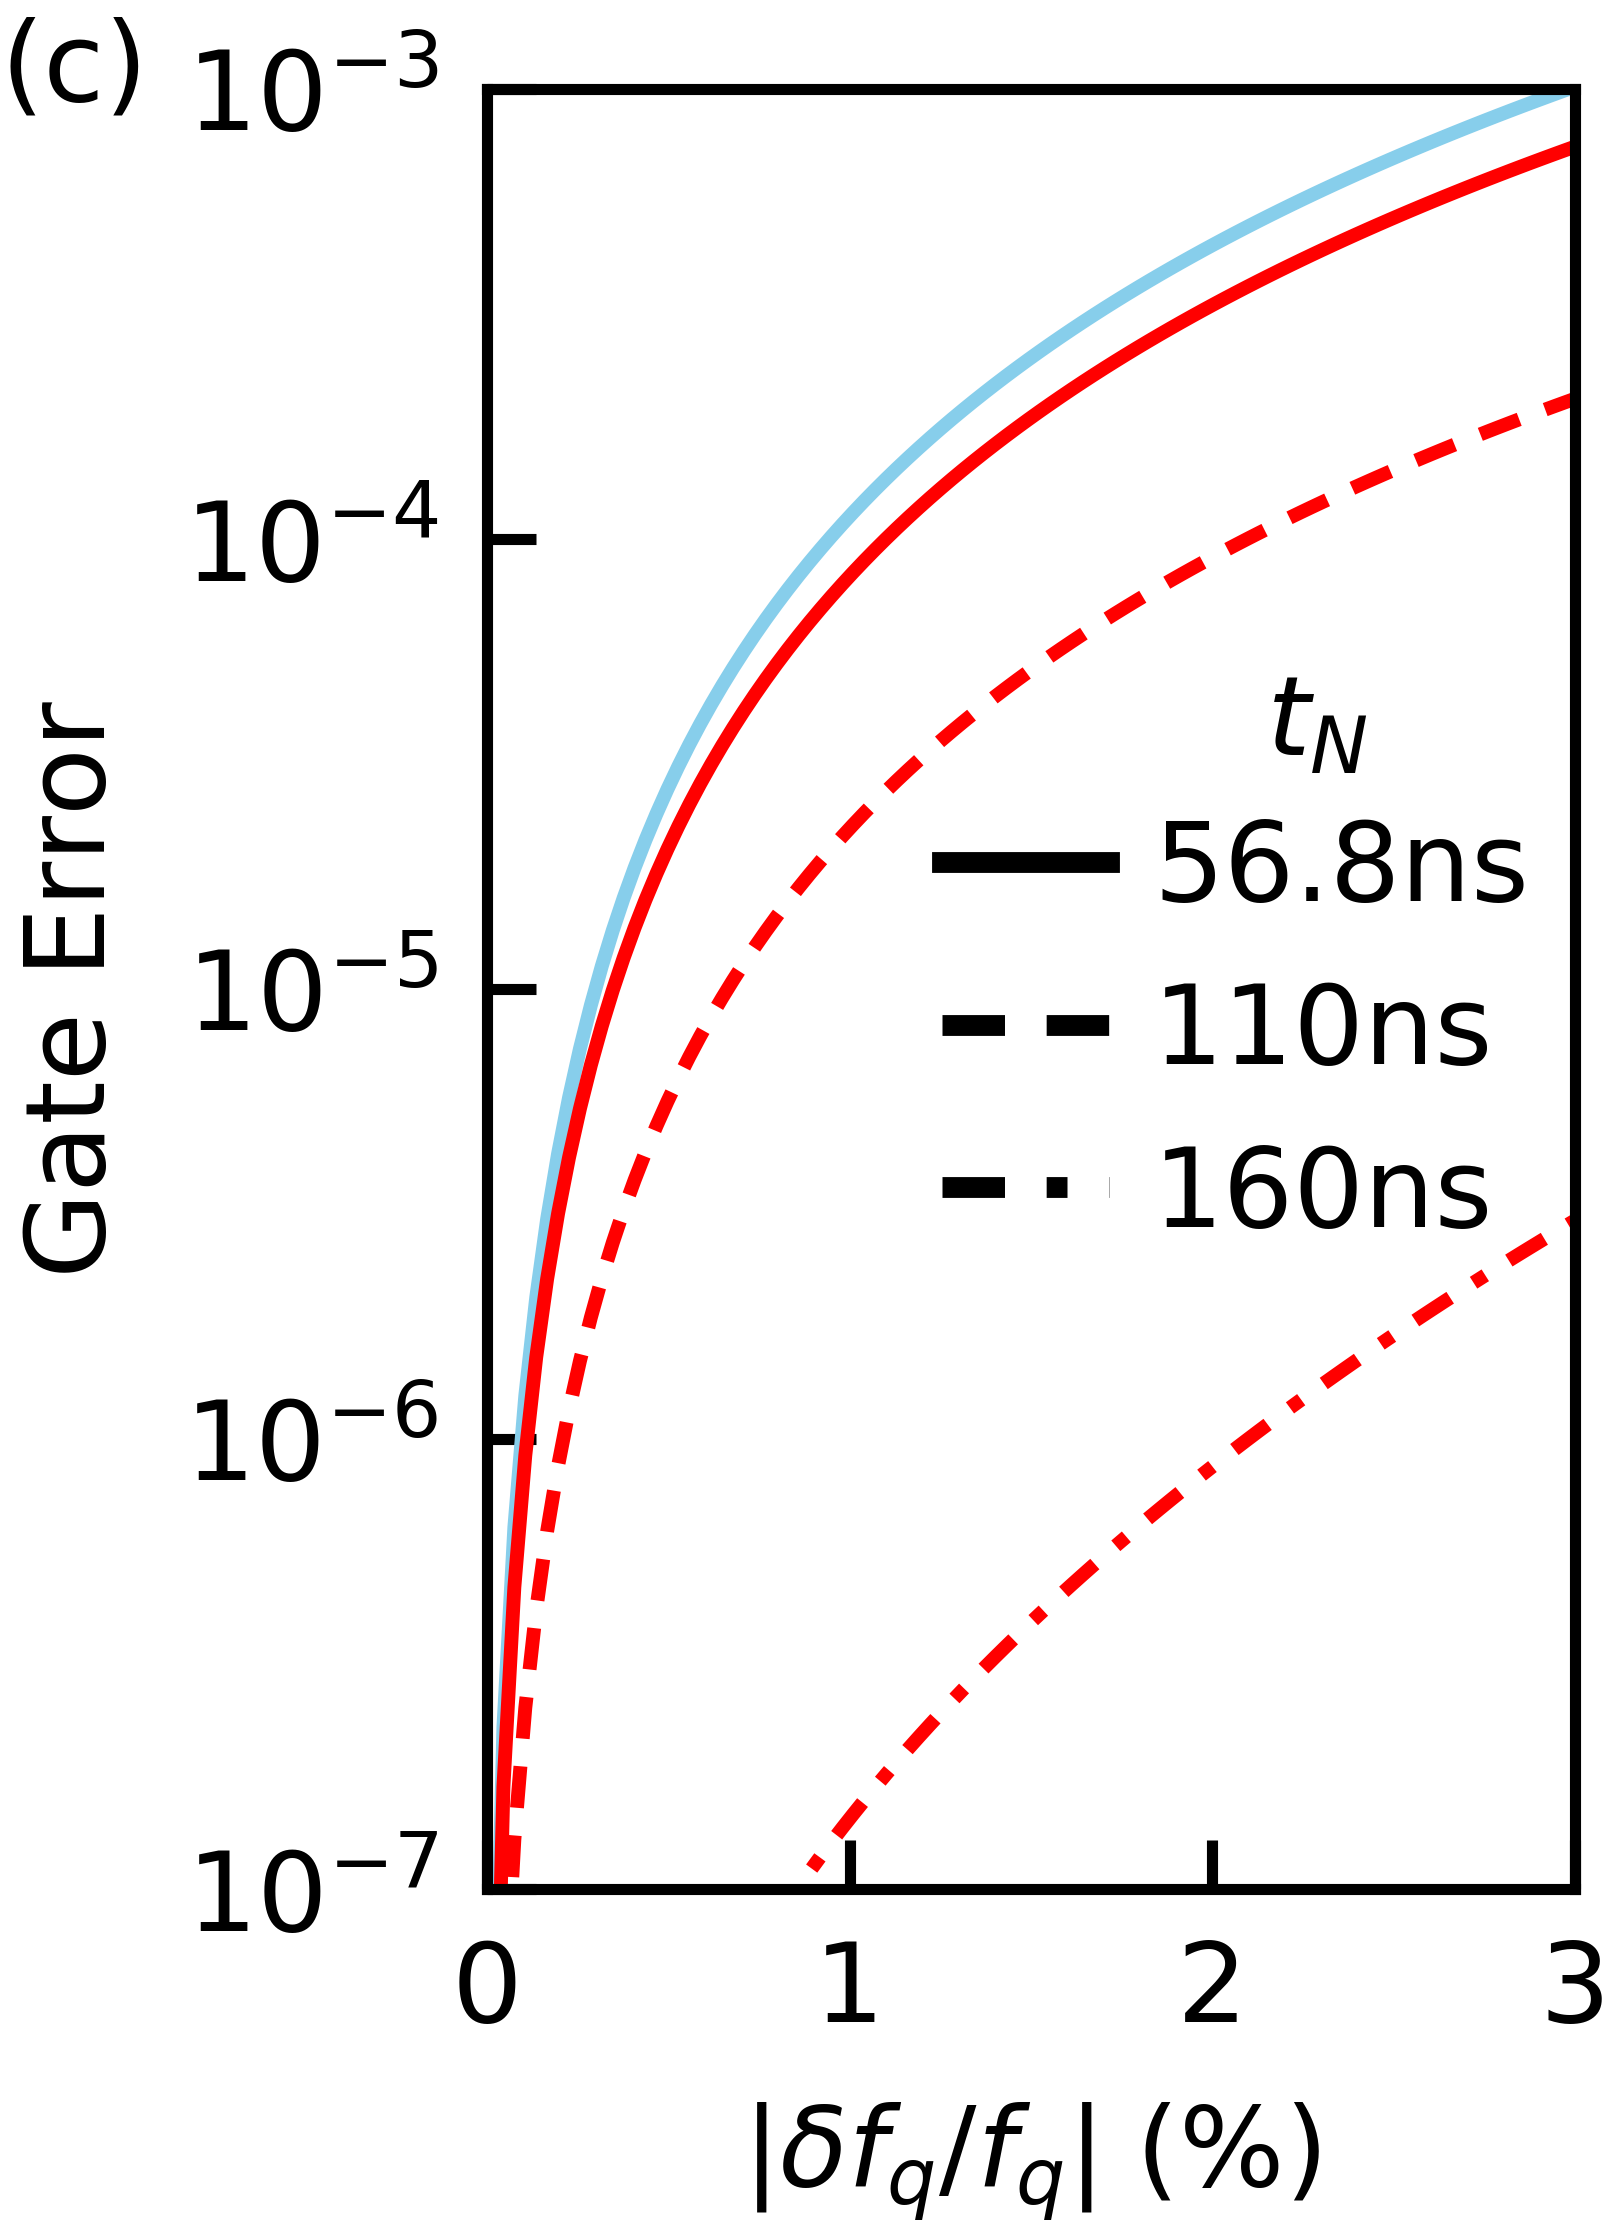
\includegraphics[width=\linewidth]{assets/f2b.png}
  \end{subfigure}
  
  \begin{subfigure}{\linewidth}
    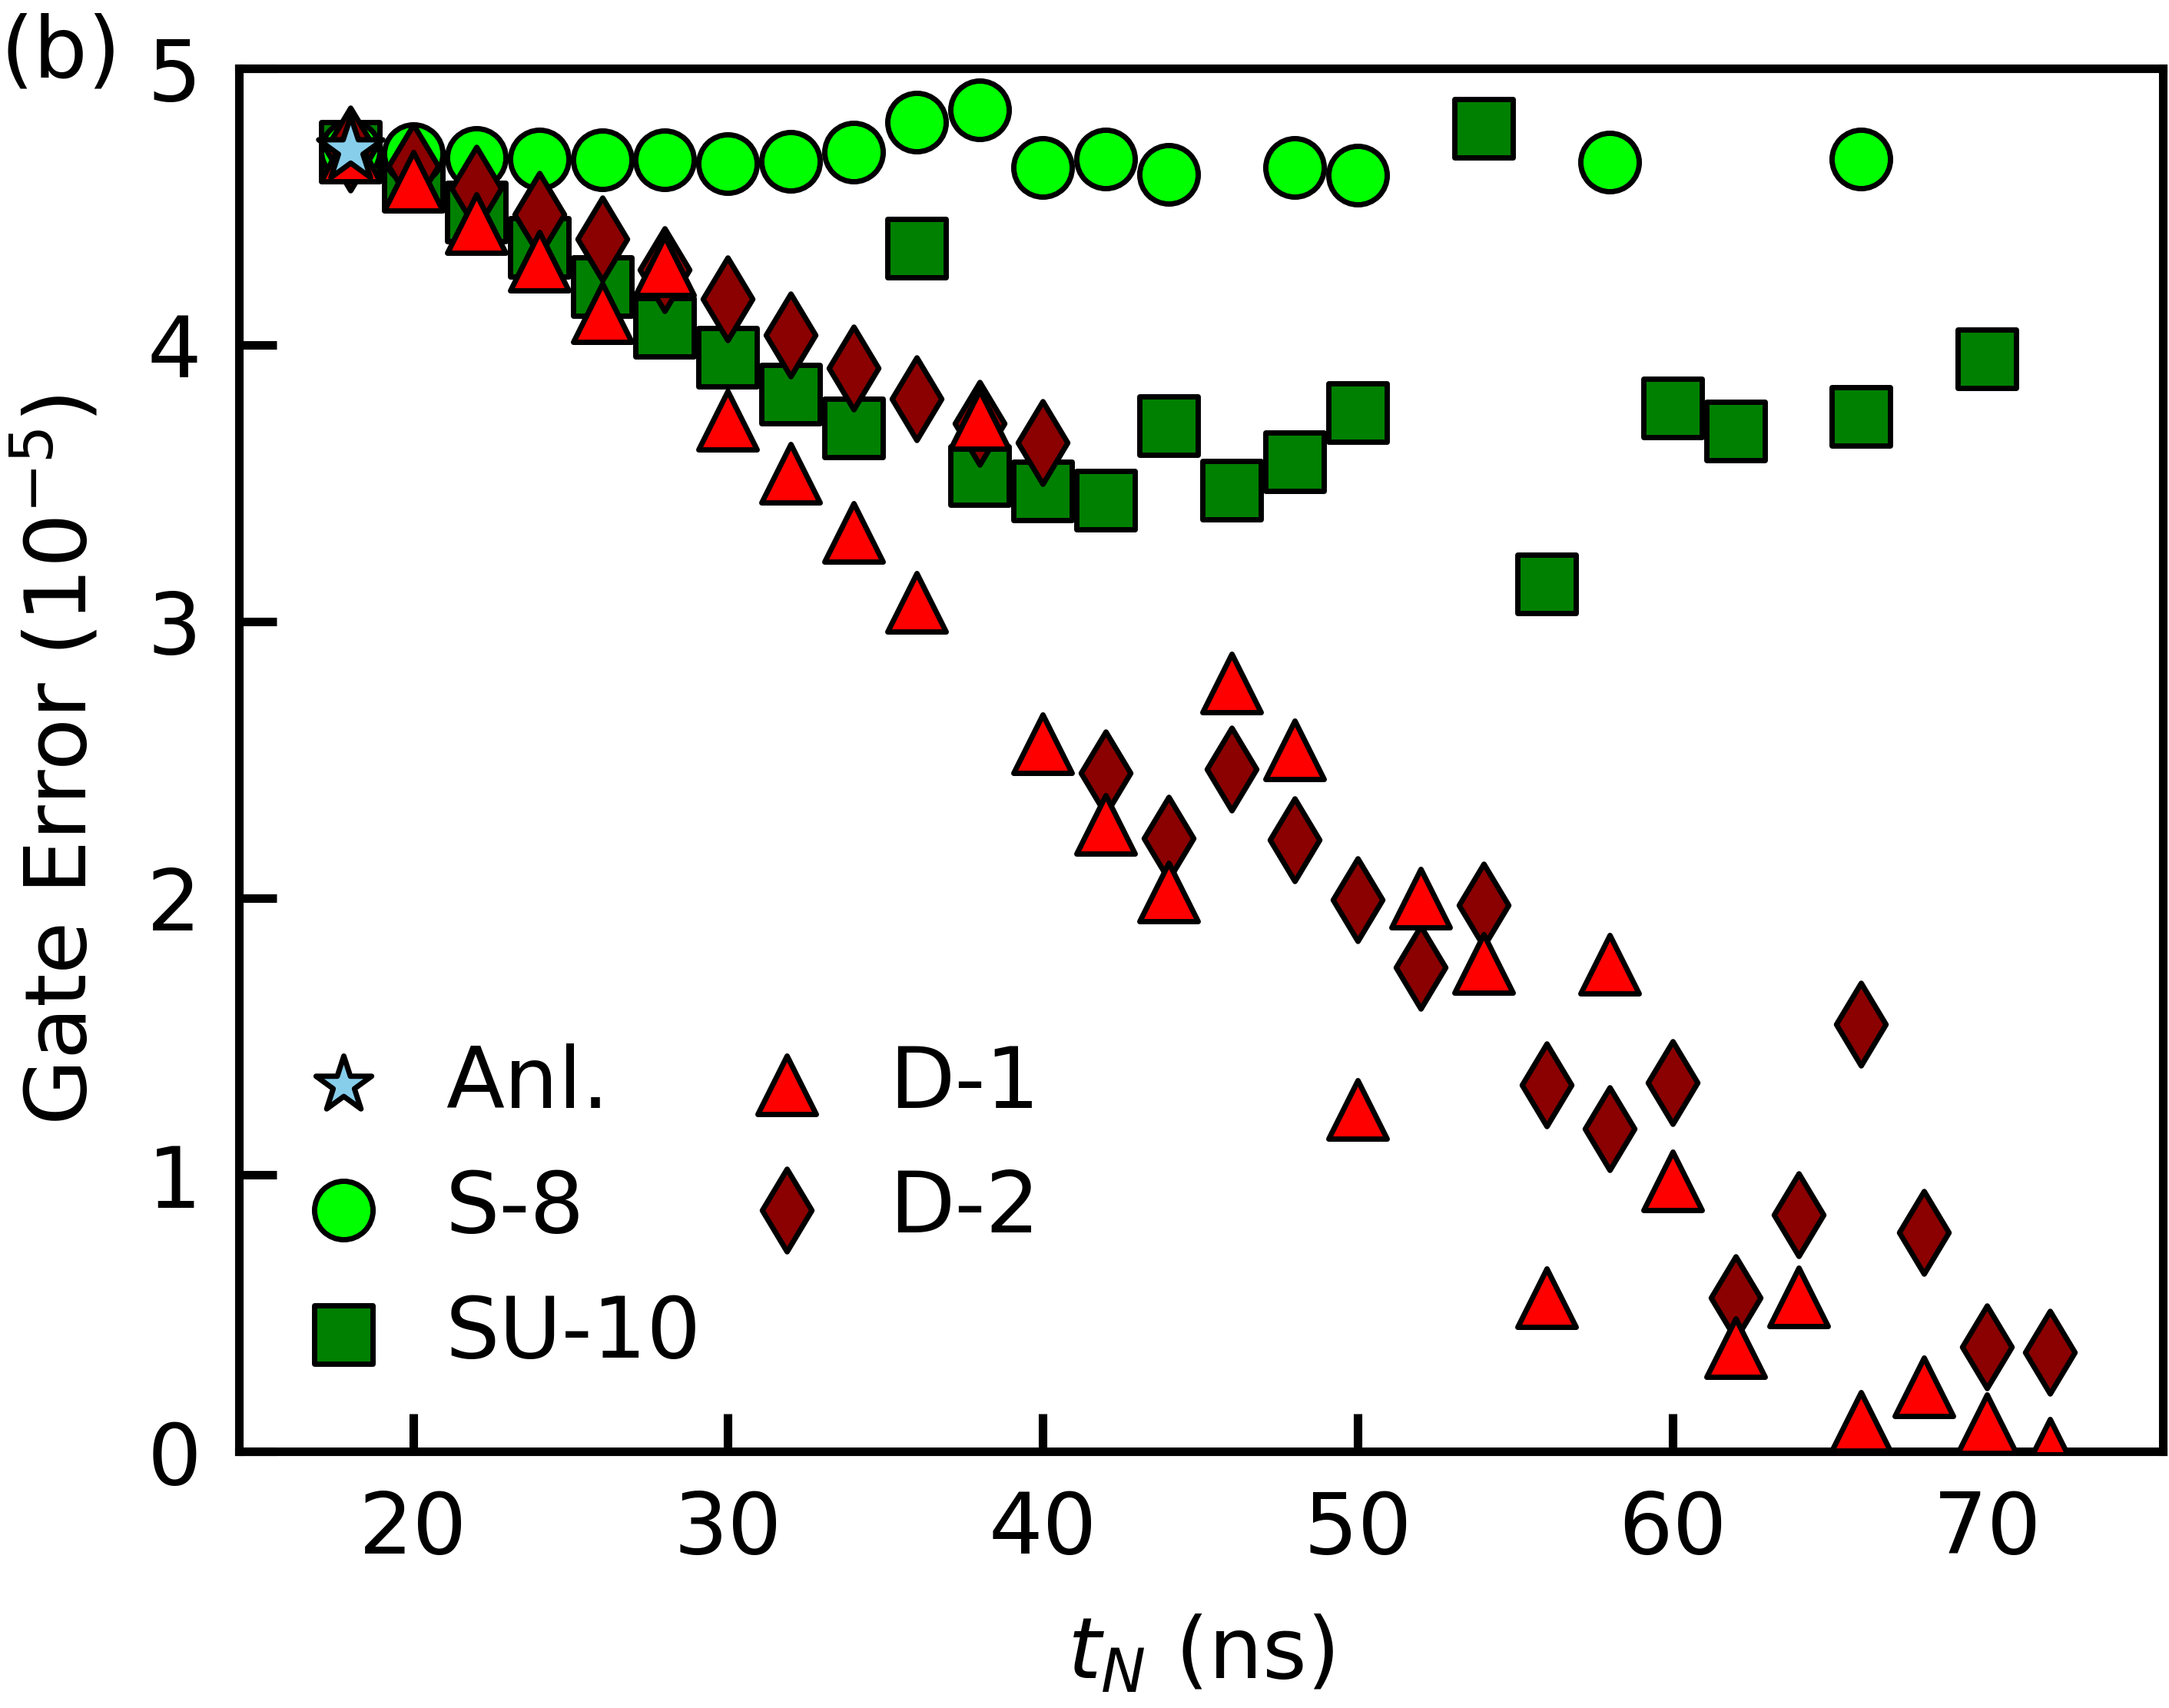
\includegraphics[width=\linewidth]{assets/f2c.png}
    \label{fig:5.1:c}
  \end{subfigure}
  
  \caption{\centering (a) $X/2$ gates constructed from the analytic, (2, 4)-point
    sampling, and (2, 3)-derivative robustness methods at a gate duration of $56.8 (ns)$.
    (b) Gate error as a function of qubit frequency detuning from the nominal frequency.
    (c) Average gate error at one standard deviation from the nominal qubit frequency as
    a function fo the gate duration.
  }
\end{figure}

%% F5.2
%% TODO: Make this figure.
\begin{figure}[ht]
  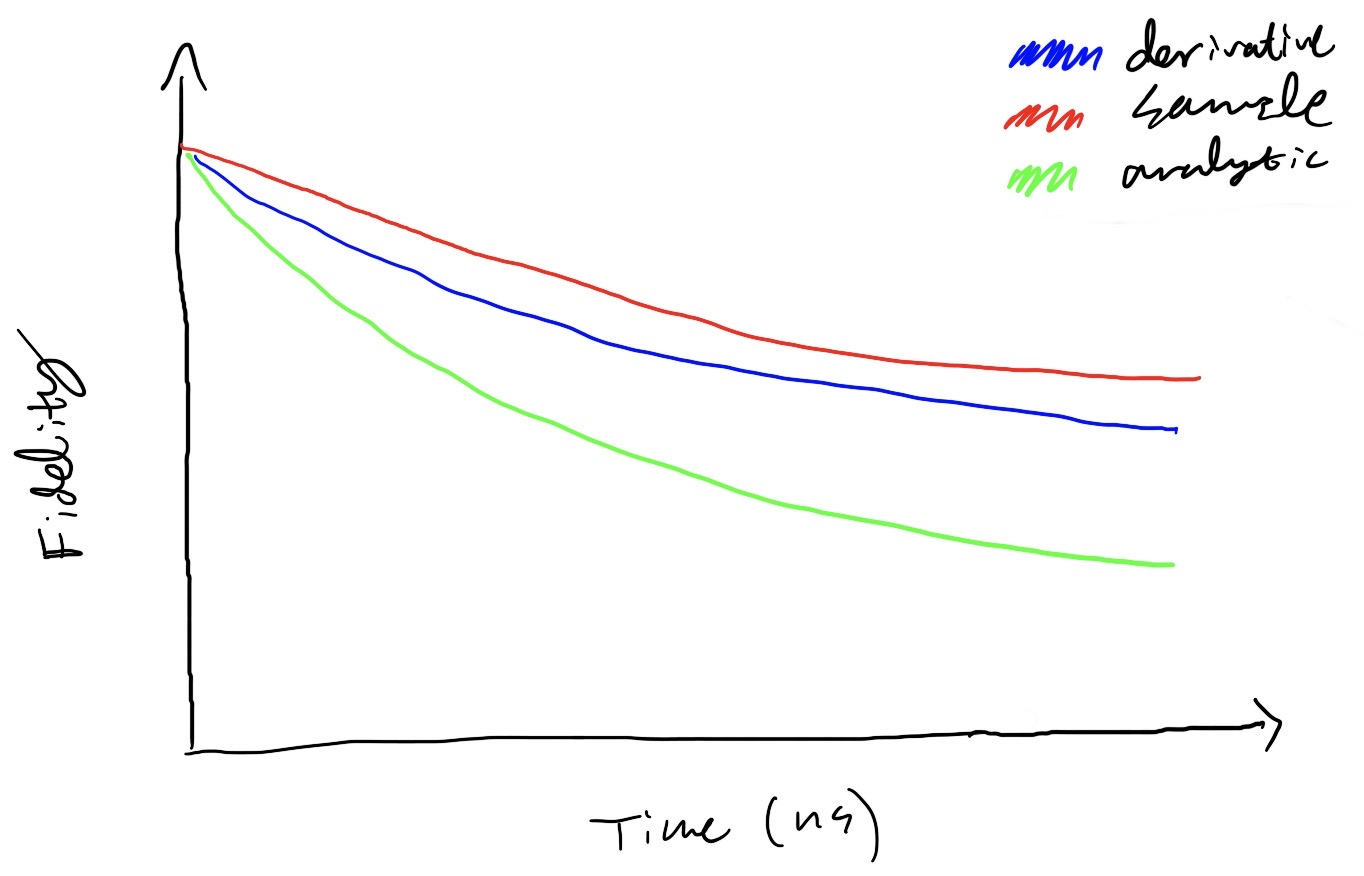
\includegraphics[width=\linewidth]{assets/t2_temp.jpg}
  \caption{Robustness to $T_{\phi}$-type noise for the
    the (2, 4)-point sampling method, (2\textsuperscript{nd}, 3\textsuperscript{rd})
    order derivative method, and B2CORPSE pulse for the $R_{x}(\pi/2)$ gate.}
\end{figure}

%% S5
\section{Robustness to Parameter Deviations}
(Strategy) For the fluxonium, pure dephasing acts
along the flux axis. Low frequency 1/$f$ noise,
Johnson-Nyquist current noise present in the flux bias
lines, and temperature dependent gain fluctuations
may cause the flux amplitude to deviate from its
desired value by an amount $\delta a$. Additionally,
residual calibration errors and fluctuations may cause
the qubit frequency to deviate from its measured value
by an amount $\delta \omega_{q}$.

System parameter
deviations are typically addressed with dynamic decoupling
sequences \cite{merrill2014progress},
the DRAG scheme \cite{krantz2019quantum}, or
geometric phase considerations
\cite{xu2020nonadiabatic} \cite{han2020experimental}.
Dynamic decoupling sequences compose rotations on the
Bloch sphere so that erroneous rotations arising due
to the parameter deviation are cancelled.
The latter two methods are inflexible. We draw on the
robust control literature to demonstrate
numerical techniques for engineering robustness
to parameter deviations.

We propose two methods for engineering robustness
to parameter deviations. The first we call the
derivative method. We draw on the intuition that
making the state evolution insensitive to changes
in the parameter ($x$) is encoded in the derivative of
the state with respect to that parameter
$\partial_{x}^{l} \ket{\psi}$.
The derviatives of the state are propgated in the
augmented state vector. Their dynamics are found by differentiating
the TDSE dynamics with respect to the parameter of interest
(see Appendix). Setting the target derivatives of the state
to zero vectors results in quadratic costs at each
knot point
${\lvert \partial_{x}^{l} \ket{\psi_{k}} \rvert}^{2}$.

The second scheme we analyze is the sampling method,
which is well studied in the robust control literature
\cite{manchester2016derivative} \cite{tronarp2016sigma}.
We add additional
states that follow deviant dynamics to the augmented
state vector. The parameters of interest
are altered by a small deviation, typically chosen
to represent the distribution of the parameter.
For example, in the 2-point sampling method we
propagate $\ket{\psi^{\pm, I}(t)}$ where
$\omega_{q}^{\pm} = \omega_{q} \pm \sigma_{\omega_{q}}$,
$\omega_{q}^{I} = \omega_{q}$.
The difference between the final states and the target
state is penalized, resulting in quadratic costs at
each knot point
${\lvert \ket{\psi^{\pm, I}_{k}} - \ket{\psi_{f}} \rvert}^{2}$

(Results) We compare the robust control
schemes to a dynamic decoupling pulse
for a single $R_{x}(\pi/2)$ gate
subject to qubit frequency detuning
($\omega_{q} \gets \omega_{q} + \delta \omega_{q}$)
to demonstrate the applicability of our techniques to mitigate
system parameter deviations.
We use a compensating for off-resonance error
(CORPSE) dynamic decoupling pulse that is optimized
to mitigate first-order error arising due to the detuning.
The pulse is composed of
three rotations about the $\hat{x}$, $-\hat{x}$, and $\hat{x}$ axes
of the Bloch sphere
designed to compensate for erroneous rotations
(see Appendix). We simulate the gate fidelity as
a function of the qubit frequency detuning for
variants of the
derivative method, sample method, and
CORPSE pulse (see Figure 2a). We also find that
increasing the gate duration allows the optimizer
to find a more robust pulse
(see Figure 2b). Increasing the order of the derivative
and sample methods requires propagating an additional quantum state
in the augmented state vector, a linear increase
in the computational complexity, but finding higher order
variants of the CORPSE family is prohibitively difficult.

Additionally, we compare the robust control
schemes to a dynamic decoupling pulse
for sequential $R_{x}(\pi/2)$ gates
subject to $T_{\phi}$ noise to demonstrate the applicability
of our techniques to mitigate noise of this type.
We simulate the gate fidelity as a function of time
for variants of the derivative method,
sample method, and B2CORPSE pulse (see Figure 3).
The B2CORPSE pulse is constructed to be robust
to qubit frequency detuning errors and
amplitude scaling errors (see Appendix).
The derivative and sampling methods are employed to
mitigate error due to qubit frequency detuning
($\omega_{q} \gets \omega_{q} + \delta \omega_{q}$)
as well as flux amplitude scaling error
($a \gets a (1 + \delta a)$).

%% S6
\section{Conclusion}
We have proposed some schemes and they work well.


\appendix
%% AA
\section{Ricatti Recursion}
This will give the reader unfamiliar with trajectory
optimization intuition for how the trajectory optimization
update scheme works and why it is better than
a more naive method.


%% AB
\section{Experiment}
We measure $T_{1}$ using the standard experiment
and $T_{2}$ using te Ramsey experiment. We fit with splines
and the data looks like fig. 3 in Helin's paper \cite{zhang2020universal}.
We measure $\omega_{q}$ and $\sigma_{\omega_{q}}$ using X method.


%% AC
\section{Dissipation Simulation}
We model dissipation using the Lindblad master
equation. 
\begin{equation}
  \frac{d}{dt} \rho = \frac{-i}{\hbar} [H, \rho] + \sum_{i = 1}^{N^{2} - 1} \gamma_{i} (L_{i} \rho L_{i}^{\dagger} - \frac{1}{2} \{L_{i}^{\dagger} L_{i}, \rho\})
\end{equation}
where $\rho = \ket{\psi}\bra{\psi}$ is the density matrix, $N = \textrm{dim}(\mathcal{H})$,
and $[\cdot, \cdot], \{\cdot, \cdot \}$ are the algebraic commutator and anti-commutator.
For longitudinal relaxation $\gamma_{1} = T_{1}^{-1} = T_{1, \uparrow}^{-1} + T_{1, \downarrow}^{-1}$
and $L_{\uparrow} = \sigma^{+}/2$,
$L_{\downarrow} = \sigma^{-}/2$
are the ladder operators $\sigma^{\pm} = \sigma_{x} \pm i \sigma_{y}$. For pure dephasing
$\gamma_{2} = T_{2}^{-1} = (2 T_{1})^{-1} + T_{\phi}^{-1}$ and
$L_{2} = (I - \sigma_{z})/2$.


%% AD
\section{Derivative Method Dynamics}
To obtain the dynamics for the derivative of the state $\partial_{x}^{l} \ket{\psi(t)}$
we differentiate the TDSE dynamics \ref{eq:tdse} with respect to the parameter of interest
($x$). Using the fluxonium hamiltonian \ref{eq:hamiltonian} we obtain the derivative of the
state with respect to the qubit frequency ($\omega_{q}$) and the flux amplitude ($a$).
Here we present the dynamics for the second derivative of the state with respect to the
qubit frequency. The case is analogous for the flux amplitude. Both $H$ and $\ket{\psi}$ are functions
of $\omega_{q}$, $a$, and $t$, but we omit the explicit dependence in notation for
brevity.
\begin{equation}
  \begin{aligned}
      \partial_{\omega_{q}} \partial_{t} \ket{\psi} &= \partial_{\omega_{q}} H \ket{\psi}\\
      &= (\partial_{\omega_{q}} H) \ket{\psi} + H (\partial_{\omega_{q}} \ket{\psi})\\
      &= \frac{\sigma_{z}}{2} \ket{\psi} + H (\partial_{\omega_{q}} \ket{\psi})
  \end{aligned}
\end{equation}
\begin{equation}
  \begin{aligned}
    \partial_{\omega_{q}}^{2} \partial_{t} \ket{\psi} &= \partial_{\omega_{q}} (\partial_{\omega_{q}} H \ket{\psi})\\
    &= (\partial_{\omega_{q}}^{2} H) \ket{\psi} + 2 (\partial_{\omega_{q}} H)(\partial_{\omega_{q}} \ket{\psi})\\
    &\quad + H (\partial_{\omega_{q}}^{2} \ket{\psi})\\
    &= \sigma_{z} (\partial_{\omega_{q}} \ket{\psi}) + H (\partial_{\omega_{q}}^{2} \ket{\psi})
  \end{aligned}
\end{equation}
The augmented state vector carries $\partial_{\omega_{q}}^{l} \ket{\psi}$
which appears explicitly in its own dynamics. Due to the dependence of $H$ on $\omega_{q}$ and $a$,
the $l$\textsuperscript{th} state derivative is coupled to the
$l - 1$\textsuperscript{th} state derivative.


%% AE
\section{Dynamic Decoupling Sequences}
Here we present the equations for constructing the CORPSE and
B2CORPSE sequences.


%% AF
\section{Complex Tensor Handling}
We use an isomorphism $\mathcal{H}(\mathbb{C}^{n}) \cong \mathcal{H}(\mathbb{R}^{2n})$
because the software we use does not support complex numbers yet.


\bibliography{refs}

\end{document}
